\chapter{Analyse} \label{chapter:analysis}

Um entscheidende Rahmenbedingungen für das Projekt festzulegen und diverse
Einflüsse auf die Entwicklung, sowie die spätere Nutzung des Systems einschätzen
zu können, wurde eine Analyse nach dem menschenzentrierten Gestaltungsprozess
durchgeführt, um Kontext und Teilnehmende einzuordnen und genauer zu verstehen.
Aufgrund der vielfältigen Veranstaltungstypen wurden die zu betrachtenden
Veranstaltungen eingegrenzt. Zudem wurden Interviews mit Veranstaltenden (V1-V2)
und Teilnehmenden  (T1-T5) durchgeführt, auf dessen Aussagen sich mit
spezifischen IDs im Verlauf der Analyse bezogen wird. Anschließend wurde eine
Organisationsanalyse durchgeführt, um die verschiedenen Phasen einer
Veranstaltung zu eruieren. Basierend auf den Ergebnissen der
Organisationsanalyse wurden eine Benutzer- und Kontextanalyse durchgeführt. Die
Zielgruppen des Frameworks wurden eruiert und für die Konzeption relevante
Besonderheiten herausgearbeitet. In einer abschließenden Kontextanalyse wurden
die verschiedenen Nutzungskontexte des Frameworks aufgezeigt und auf die mit
ihnen einhergehenden Herausforderungen eingegangen.


\section{Datenquellen}

Im Rahmen der Analyse wurden verschiedene Datenquellen genutzt. Eingangs wurde
eine wissenschaftliche Literaturrecherche am 11.08.2021 durchgeführt.
Verschiedene vergleichbare Projekte wurden im Rahmen einer Internetrecherche
ermittelt. Unter anderem wurden die Ausarbeitung und Evaluation der
EMI-Award-App als Quellen genutzt. Zudem wurden Interviews mit Veranstaltenden
und Teilnehmenden durchgeführt. \\
Zur Literaturrecherche wurden die digitalen Bibliotheken ACM Digital Library
\footnote{\url{https://dl.acm.org/}} und Google Scholar
\footnote{\url{https://scholar.google.de/}} genutzt. Es wurden Begriffe aus den
Bereichen Event Management (\emph{Event Management, Event Evaluation, Event
Experience, Event Tracking}) und UX (\emph{Attention Economy, Attention
Management, Information Overload, Digital Burnout, Overchoice, Web Animation,
Animation UX, UX Micro Interaction, Animation Usability}) zur Suche verwendet.
\\
Die Interviews mit Veranstaltenden und Teilnehmenden wurden qualitativ und
semistrukturiert, mithilfe eines dafür entworfenen Interviewleitfadens (siehe
\autoref{appendix:interview}), durchgeführt. Bei den Veranstaltenden handelt es sich um Personen mit
praktischer Erfahrung in der Organisation von Veranstaltungen. In Tabelle
\ref{table:ver-soz} und Tabelle \ref{table:teil-soz} sind Details zu den
befragten Personen aufgelistet. Die IDs der interviewten Personen werden im
Verlauf der Analyse referenziert.

\begin{table}[htpb]
    \def\arraystretch{1.25}
    \centering
    \caption{Soziodemografische Daten der Veranstaltenden}
    \label{table:ver-soz}
    \begin{tabular}{lcl}
        \uzlhline
        \uzlemph{ID} & \uzlemph{Alter} &
        \uzlemph{Vorerfahrung}                         \\
        \uzlhline V1 & 40 - 59 J.      & Verschiedene
        Veranstaltungen, verteilt über 11 Jahre        \\
        V2           & 18 - 25 J.      & Mehrere große
        Veranstaltung (>2000 Teilnehmende)             \\
        \uzlhline
    \end{tabular}
\end{table}

\begin{table}[htpb]
    \def\arraystretch{1.25}
    \centering
    \caption{Soziodemografische Daten der Teilnehmenden}
    \label{table:teil-soz}
    \begin{tabular}{lccl}
        \uzlhline
        \uzlemph{ID}                     & \uzlemph{Alter}     &
        \uzlemph{EMI-Award-App genutzt?} & \uzlemph{Tätigkeit}
        \\
        \uzlhline T1                     & 18 - 25 J.          & j
                                         & Student:in              \\
        T2                               & 18 - 25 J.          & j
                                         & Student:in              \\
        T3                               & 18 - 25 J.          & j
                                         & Student:in              \\
        T4                               & 18 - 25 J.          & n
                                         & Student:in              \\
        T5                               & 40 - 59 J.          & n
                                         & Berufstätig             \\
        \uzlhline
    \end{tabular}
\end{table}


\section{Definition: Veranstaltung} \label{sec:analysis-def}

Bevor die verschiedenen Aufgaben, Probleme und Benutzergruppen analysiert werden
können, müssen Umfang und Typ der Veranstaltung festgelegt werden. In der
Literatur sind verschiedene Definitionen zum Begriff „Veranstaltungen“ zu
finden, welche sich in Umfang und Inhalt unterscheiden. Die räumliche und
zeitliche Dimension von Veranstaltungen ist sehr flexibel. \textcite{Getz2007}
definiert Veranstaltungen als zeitliche Phänomene. Im Gegensatz zu ungeplanten
Veranstaltungen wird bei geplanten Veranstaltungen das Veranstaltungsprogramm
oder der zeitliche Ablauf im Allgemeinen detailliert geplant und im Voraus
bekannt gemacht. Geplante Veranstaltungen sind in der Regel auch auf bestimmte
Orte beschränkt, wobei es sich um eine bestimmte Einrichtung, eine sehr große
Freifläche oder verschiedene Orte handeln kann. \textcite{Bladen2012} definieren
Veranstaltungen als zeitlich begrenzte und zweckgebundene Zusammenkünfte von
Menschen.

Im Rahmen dieser Arbeit werden insbesondere Veranstaltungen betrachtet, welche
in ihrer zeitlichen Dimension von wenigen Stunden bis auf mehrere Wochen
beschränkt sind und räumlich verteilt stattfinden. Konkret verteilen sich die
Aktivitäten der Veranstaltung auf einen größeren Raum. Dies kann mindestens die
Aufteilung auf verschiedene Räumlichkeiten sein, bis hin zur Verteilung über
verschiedene Stadtteile.


\section{Organisationsanalyse} \label{sec:analysis-org}

% Masterarbeit_Holtz  Aufgabenanalyse!!!
Die hier analysierte Vorgehensweise in der Organisation von Veranstaltungen
basiert auf dem EMBOK-Model \cite{Silvers2013} und den Aussagen der interviewten
Veranstaltenden (V1 - V2). Typischerweise lässt sich die Organisation von
Veranstaltungen in 5 Phasen (\autoref{fig:embok-phases}) gliedern: Initiation,
Planung, Umsetzung, Durchführung und Schließung. Die Vorgehensweise in den
Phasen gestaltet sich wie folgt:

\begin{enumerate}
    \setlength{\itemsep}{1em}
    \item \textbf{Initiation} \\
          Es wird recherchiert, um ein Konzept zu erstellen und zu validieren.
          Umfang und Kontext sowie Ziele und Aufgaben werden festgesetzt.\\
    \item \textbf{Planung} \\
          Anforderungen und Spezifikationen werden festgehalten. Hierzu zählen
          die stattfindenden Aktivitäten, sowie die Art der Organisation und
          erforderliche Ressourcen.
    \item \textbf{Umsetzung} \\
          Alle für die Veranstaltung benötigten Waren und Dienstleistungen
          werden in Auftrag gegeben und koordiniert. Der Fokus liegt unter
          anderem auf der Überwachung und Überprüfung des Umfangs und Zeitplans,
          sowie der Kosten und Qualität.
    \item \textbf{Durchführung} \\
          Die veranstaltungsbezogenen Aktivitäten werden aufgenommen. Ab Beginn
          dieser Phase ist der Handlungsrahmen stark eingeschränkt, wodurch der
          Fokus auf der Überwachung der Veranstaltung liegt.
    \item \textbf{Schließung} \\
          Nach Abschluss der Veranstaltung werden Daten gesammelt, ausgewertet
          und weitergegeben. Das Ziel ist die Dokumentation der Erkenntnisse für
          weitere Veranstaltungen.
\end{enumerate}

\begin{figure}[htpb]
    \centering
    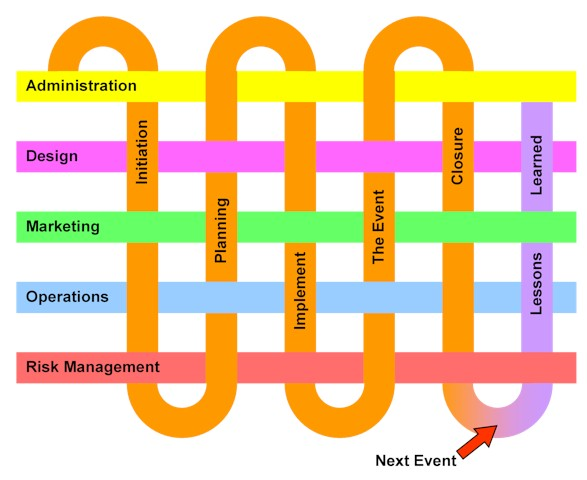
\includegraphics[width=\textwidth]{embok_phases.jpg}
    \caption{Die Phasen der Veranstaltungsorganisation \cite{Silvers2013b}. Die
        verschiedenen Phasen (vertikal) bilden die Grundlage einer
        Veranstaltung. Verwoben sind diese mit Wissensdomänen (horizontal).
        Sollte einer der Fäden verschwinden, wird das gesamte Geflecht
        geschwächt.}
    \label{fig:embok-phases}
\end{figure}

In dieser Arbeit wird vor allem die Unterstützung ab der Umsetzung (vgl.
\autoref{sec:goals}) adressiert, weshalb insbesondere die Phasen „Umsetzung“,
„Durchführung“ und „Schließung“ näher betrachtet werden.

\subsection{Umsetzung} \label{ssec:analysis-org-umsetzung}

In dieser Phase werden die herausgearbeiteten Pläne umgesetzt. Hierbei werden
Umfang, Zeitpläne, Kosten, Kommunikation und Risiken überwacht und kontrolliert,
um die plangemäße Ausführung sicherzustellen. Weitere Arbeits-/Hilfskräfte
werden engagiert, um bei der Umsetzung mitzuwirken. Für den Erfolg der
Veranstaltung ist die effektive Kommunikation wichtig. Um diese zu
gewährleisten, muss eine Kommunikationsinfrastruktur für Organisierende,
Mitwirkende und externe Dienstleister eingeführt werden. Hilfskräfte müssen in
die Kommunikationsinfrastruktur eingewiesen werden. Aufgrund von mangelnden
technischen Fähigkeiten können bei komplexeren Infrastrukturen Probleme
auftreten (V2).

\subsection{Durchführung} \label{ssec:analysis-org-durchfuehrung}

Mit Beginn der Durchführung ändert sich die Dynamik der Veranstaltung bedeutend.
Aufgrund der Anwesenheit von Teilnehmenden sind tiefgreifende Änderungen nun
nicht mehr möglich und beschränken sich auf die Behebung von kleinen Problemen
(V2). Hingegen wird die wichtigste Aufgabe die Überwachung der Veranstaltung.
Unter besonderer Beobachtung stehen logistische Tätigkeiten, sowie unerwartet
auftretende Probleme~(V1, V2). Diese können u. a. durch Teilnehmende,
stattfindende Aktivitäten oder die Umgebung der Veranstaltung ausgelöst werden.
\\
Während Probleme, welche die Durchführung der Veranstaltung direkt
beeinträchtigen könnten, streng beobachtet und behoben werden, stehen die
Interaktionen und Erfahrungen der Teilnehmenden zunächst im Hintergrund.
Abgesehen von kritischem Feedback, wird die Erfahrung erst während der
Schließung erfasst und ausgewertet (V2).

\subsection{Schließung} \label{ssec:analysis-org-schliessung}

% Bedeutung Evaluation aus Finischen Case S.57-59 Mischung Quantitativ &
% Qualitativ Evaluation S.61

Zur Schließung der Veranstaltung wird die Evaluation zur bedeutendsten Aufgabe.
Feedback und Daten werden von organisierender Seite gesammelt. Hierbei wird
zwischen \textit{weichen} und \textit{harten Daten} unterschieden. Harte Daten
bestehen aus Teilnehmerzahlen, Andrang an verschiedenen Aktivitäten, Dauer,
Einkommen und weiteren zählbaren Merkmalen. Im Vergleich dazu bestehen weiche
Daten u. a. aus Beschwerden, Konflikten, Problemen, Komplimenten, Reaktionen und
Empfehlungen. Mitwirkende, Hilfskräfte und die Organisierenden werden meist dazu
in einer Nachbesprechung befragt (V1, V2). Das Feedback von Teilnehmenden wird
oft nur passiv vor Ort vom Personal erfasst und weitergegeben oder beschränkt
sich auf Familie und Freunde (V2). Die erfassten Erkenntnisse werden
dokumentiert, um auf das Wissen in der nächsten Veranstaltung zurückgreifen zu
können.

\newpage

\section{Benutzeranalyse} \label{sec:analysis-user}

Um die Funktionen des Frameworks zielgruppengerecht gestalten zu können, werden
in diesem Abschnitt die Benutzergruppen des Frameworks eruiert und näher
analysiert. Zu den Benutzergruppen gehören Veranstaltende, sowie Teilnehmende
einer Veranstaltung.

\subsection{Veranstaltende} \label{ssec:analysis-user-v}

Inzwischen existieren weltweit tausende Einrichtungen, welche formale
Qualifikationen und Ausbildungen im Veranstaltungsmanagement anbieten. Jedoch
sind diese Qualifikationen nicht einheitlich festgelegt, was zu
unterschiedlichen Schwerpunkten, Umfang, Vermittlungsart und letztendlich
erworbenen Qualifikationen führt \cite{Bladen2012}. In Deutschland gibt es den
anerkannten Ausbildungsberuf des/der Veranstaltungs\-kaufmann/-frau. Die
Aufgaben sind hierbei die Konzipierung und Organisation des kaufmännischen
Aspektes von Veranstaltungen \cite{Kultusministerkonferenz2001}. Die Aufgaben
von Event Manager:innen umfassen zusätzlich die allgemeine Organisation und
Aufgaben im Marketing \cite{BundesagenturfurArbeit2021}. Jedoch ist die
Berufsbezeichnung „Event Manager/in“ rechtlich nicht geschützt. \\
Zudem bedarf es in Deutschland keiner formalen Qualifikation, um eine
Veranstaltung beliebiger Größe zu organisieren. Dementsprechend können keine
bestimmten Qualifikationen für Veranstaltende angenommen werden.

\subsection{Teilnehmende} \label{ssec:analysis-user-t}

Die Teilnehmenden einer Veranstaltung unterscheiden sich stark in ihren
soziodemografischen Daten je nach Typ der Veranstaltung. Im Kontext der
vorliegenden Arbeit sind besonders Alter, Technikaffinität und körperliche,
seelische, geistige oder Sinnesbeeinträchtigungen zu beachten. Im Rahmen der
weiteren Analyse wird das Alter der Teilnehmenden auf 16 - 60 J. begrenzt. Zudem
wird die sichere grundlegende Umgangsweise mit einem Smartphone vorausgesetzt.

Da die Literatur zu Event Management ihren Fokus auf die Organisation legt, sind
nur wenig Informationen zur Sicht der Teilnehmenden und ihren Charakteristika
vorhanden. Als Messwerte für eine erfolgreiche Veranstaltung werden meist
geschäftsrelevante Werte wie z. B. verkaufte Tickets, Teilnehmerzahlen, Umsatz
oder öffentliche Aufmerksamkeit verwendet, welche wenig über die Erfahrung der
Teilnehmenden aussagen \cite{Getz2007}. In Interviews wurden die Teilnehmenden
gebeten zu begründen, was eine gewählte Veranstaltung zu ihrem persönlichen
Favoriten macht (vgl. \autoref{table:teil-fav}).

\begin{table}[htpb]
    \def\arraystretch{1.25}
    \centering
    \caption{Merkmale von positiv empfundenen Veranstaltungen}
    \label{table:teil-fav}
    \begin{tabular}{ll}
        \uzlhline
        \uzlemph{Grund}               & \uzlemph{ID} \\
        \uzlhline  Sozialer Austausch & T1, T2       \\
        Innovative Technik            & T2           \\
        Persönliche Bindung           & T4           \\
        Gute Musik                    & T3           \\
        Einfache Wegfindung           & T5           \\
        Neues Wissen                  & T5           \\
        \uzlhline
    \end{tabular}
\end{table}

\section{Kontextanalyse} \label{sec:analysis-context}

In diesem Abschnitt werden der zeitliche und räumliche Kontext untersucht. Aus
den Ausführungen in \autoref{sec:goals} geht der Fokus auf die Unterstützung von
Veranstaltenden und Teilnehmenden hervor. Die Unterteilung der Benutzergruppen,
wie in \autoref{sec:analysis-user} beschrieben, ist zu beachten. Hieraus ergeben
sich unterschiedliche räumliche und zeitliche Kontexte für Veranstaltende und
Teilnehmende. Zusätzlich werden die Herausforderungen des Kontextes erfasst.

Die Unterstützung der Veranstaltenden findet in verschiedenen Phasen der
Organisation statt. Der zeitliche Kontext kann in „vor, während und nach“ einer
Veranstaltung unterteilt werden (vgl. \autoref{sec:analysis-org}). Vor der
Durchführung einer Veranstaltung ist insbesondere die Vorbereitung von
Aktivitäten und Absicherung von Dienstleistungen oder Waren wichtig. Je nach
Größe der Veranstaltung können eine Vielzahl von Menschen an der Organisation
beteiligt sein. Meist sind verschiedene digitale Tools oder Plattformen zur
Kommunikation erforderlich, um sich mit allen Veranstaltenden zu verständigen
(V2). Hier kann es zu Herausforderungen kommen, auch Menschen mit geringem
Technikverständnis einzuweisen (V2). \\
Während der Veranstaltung hingegen findet ein starker Fokuswechsel auf die
Beobachtung und schnelle Behebung von Problemen statt (V1). Hierbei besteht der
Bedarf kleine Änderungen noch einfacher vornehmen zu können (V1). Aber auch der
Kontakt zu Teilnehmenden spielt eine große Rolle. Jedoch ist dieser während
einer Veranstaltung meist nur gering (V1, V2). Zudem mangelt es bei räumlich
verteilten Veranstaltungen an Möglichkeiten ein Gruppengefühl zu erzeugen (V1).
\\
Nach einer Veranstaltung sind die Datensammlung und Auswertung, sowie der
Wissenstransfer von Bedeutung. Der Kontakt zu Teilnehmenden fällt hier ebenfalls
sehr schwer (V1) oder wird ausgelassen (V2).

Auch beschränken sich die betrachteten Veranstaltungen während der Durchführung
auf den in \autoref{sec:analysis-def} beschriebenen örtlichen Bereich, woraus
sich ein weitestgehend unbeschränkter räumlicher Kontext ergibt. Hierbei stellt
die Übersicht über die Veranstaltung ein Problem dar. Gerade bei räumlich
größeren Veranstaltungen gibt es keine direkte Übersicht über die Teilnehmenden
(V1). Oft werden für die Datensammlung nur Schätzungen verwendet (V2). Jedoch
ist die Reichweite ein wichtiger Indikator für Veranstaltende (V1). Allgemein
besteht die Datensammlung in der Nachbesprechung aus Aussagen von
Veranstaltenden oder deren Angehörigen und Freunden (V2). \\
Vor und nach der Veranstaltung werden komplexe Informationen eingetragen oder
ausgewertet. Da die Bildschirmgröße einen großen Einfluss auf die effiziente
Verarbeitung von Informationen hat \cite{Ni2006}, wird hierfür von einem
Arbeitsplatzsystem ausgegangen. Somit ergibt sich ein räumlich eingeschränkter
Kontext vor und nach der Veranstaltung. Folglich wird während der Veranstaltung
ein mobiles System zur Überwachung benötigt, wobei die Bedingungen vor und nach
der Veranstaltung ein stationäres System befürworten.

Für Teilnehmende ist der Kontext ebenfalls in „vor, während und nach“ der
Veranstaltung aufgeteilt. Der zeitliche Kontext während der Veranstaltung ist
hierbei am bedeutendsten. Auch für Teilnehmende gilt der in
\autoref{sec:analysis-def} beschriebene örtliche Bereich, woraus sich ebenfalls
ein unbeschränkter räumlicher Kontext ergibt. Folglich muss das System für die
Teilnehmenden mobil einsetzbar sein. Hierbei ist zu beachten, dass in Interviews
mit Teilnehmenden festgestellt werden konnte, dass Schwierigkeiten in der
Navigation von Veranstaltungen zu finden sind. Daher besteht die Nachfrage nach
einer Unterstützung in der Wegfindung und eine Übersicht über die Veranstaltung
(T1, T2, T5). Diese Unterstützung kann zum Beispiel ein Event-Assistent umfassen
(T2).

Des Weiteren konnte sowohl durch Teilnehmende, als auch durch Veranstaltende
erfasst werden, dass Personen mit körperlichen Einschränkungen durch technische
Unterstützung besser oder womöglich überhaupt an Events teilnehmen können (bspw.
Gebärdensprache in Form von Videos, Videos für Blinde, etc.).

\section{Analyse des bestehenden Systems} \label{sec:analysis-old}

An dieser Stelle wird die Implementation und Evaluation der
\textit{EMI-Award-App} vorgestellt \cite{Canzler2021}, welche die Grundlage des neuen Systems bildet.

% Tech-Stack
%   - Hat sich größten teils bewährt
%   - Web-App mit PWA Funktionalität

% Mockups
%   - Bereits getestet
%   - Grobe Struktur beibehalten

\subsection{Analyse der Funktionalitäten} \label{ssec:analysis-old-funk}

Die Funktionalitäten der EMI-Award-App gliedern sich in zwei Kategorien:
Funktionalitäten für Teilnehmende und Funktionalitäten für Veranstaltende. Im
Folgenden wird zunächst die Seite der Teilnehmenden beschrieben und anschließend
auf die Möglichkeiten der Veranstaltenden eingegangen.

Die \textit{EMI-Award-App} ermöglicht das augmentierte Besuchen, Einsehen und
Bewerten der EMI-Award-Projekte und bildet die Grundlage dieser Arbeit (vgl.
\autoref{sec:goals}). Speziell werden dafür an den Projekt-/Stationsstandorten
QR-Codes bereitgestellt, welche mithilfe eines QR-Code-Readers oder einer
Kamerafunktion, welche in der App integriert ist, gescannt werden können (\autoref{fig:emi-qr-code}).

% Speziell wurden dafür an verschiedenen Standorten Schilder
% mit QR-Codes angebracht, welche mit einem QR-Code-Reader oder der App gescannt
% werden konnten (vgl. \autoref{fig:emi-qr-code}).

\begin{figure}[htpb]
    \centering
    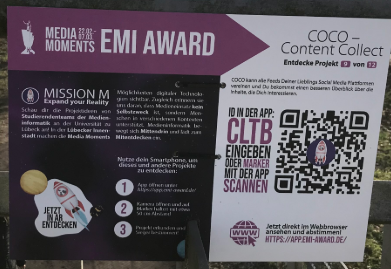
\includegraphics[width=.8\linewidth]{emi_schild.png}
    \caption{Schild eines Projektstandortes mit QR-Code}
    \label{fig:emi-qr-code}
\end{figure}

Beim ersten Aufruf der App wird dem Nutzenden eine kurze Einführung in die App
und ihre Rahmenbedingungen gegeben. Dies geschieht über eine interaktive
Slideshow. Nach dem Bestätigen der letzten Slide werden Nutzende zur
interaktiven Karte geführt (\autoref{fig:emi-intro-map}). Auf dieser werden die
Projektstandorte durch verschiedenfarbige Icons von Planeten
(\textgraphics{emi_planet.png}) dargestellt. Durch das Antippen eines Standorts
wird eine Kurzinformation, in Form eines Pop-ups, zum jeweiligen Projekt
angezeigt. Außerdem wird der Standort des Nutzenden angezeigt, insofern die
Berechtigungen dazu gegeben werden.

\begin{figure}[htpb]
    \begin{minipage}{.5\textwidth}
        \centering
        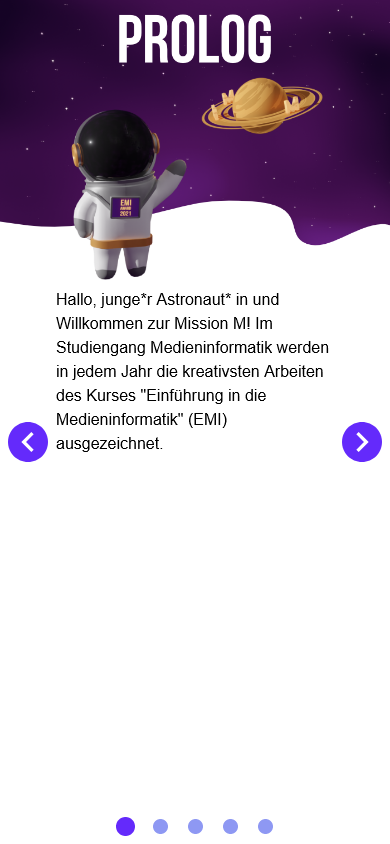
\includegraphics[width=.6\linewidth]{emi_prolog.png}
    \end{minipage}%
    \begin{minipage}{.5\textwidth}
        \centering
        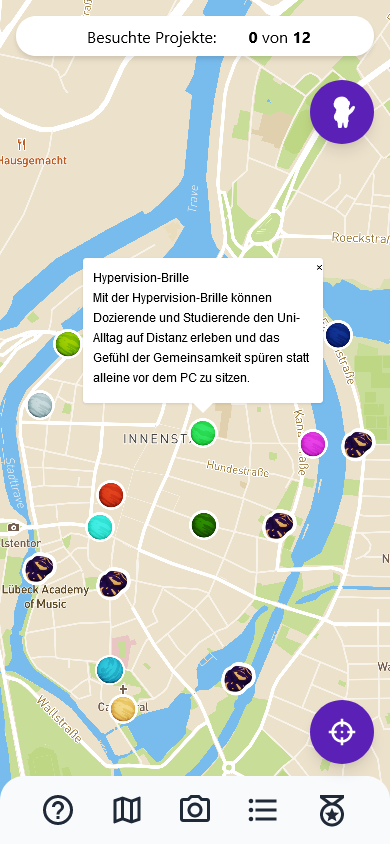
\includegraphics[width=.6\linewidth]{emi_map.png}
    \end{minipage}
    \caption{Einführung und interaktive Karte mit Projektstandorten}
    \label{fig:emi-intro-map}
\end{figure}

Um die vollständigen Informationen eines Projekts einzusehen, muss der
Standort erst virtuell besucht werden. Dies geschieht über das Scannen des
QR-Codes auf dem Schild des Standorts (\autoref{fig:emi-qr-code}) oder der
manuellen Eingabe eines spezifischen Codes. Nach erfolgreichem Scannen oder
Eingeben des Codes wird eine virtuelle Szene angezeigt. In dieser muss ein
Planet gesucht und angetippt werden, um den Vorgang abzuschließen (\autoref{fig:emi-ar}). Je nach benutztem Gerät wird die Szene per \ac{AR} oder \ac{VR} angezeigt. Zudem wird die Anzahl der
besuchten Standorte in der Karten- und Projektansicht anhand eines
Fortschrittsbalkens angezeigt. Die vollständigen Informationen der Projekte
enthalten mediale Inhalte, eine detaillierte Beschreibung und die Autoren des
Projekts. Zusätzlich kann das Projekt mit einer vorgegebenen Auswahl bewertet
werden (\autoref{fig:emi-project}).

\begin{figure}[htpb]
    \begin{minipage}{.5\textwidth}
        \centering
        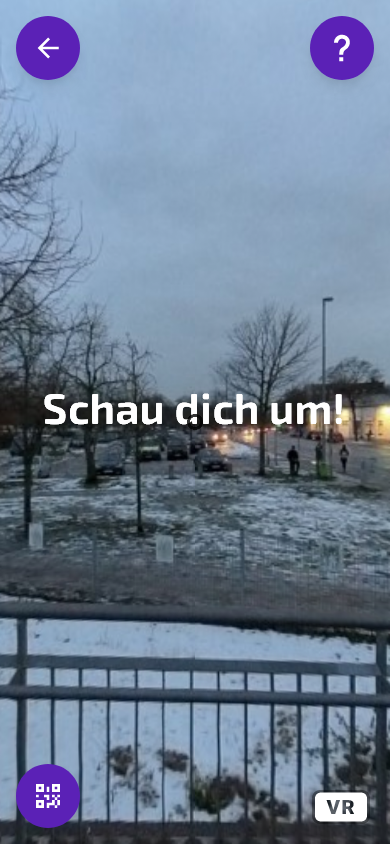
\includegraphics[width=.6\linewidth]{emi_ar-1.png}
    \end{minipage}%
    \begin{minipage}{.5\textwidth}
        \centering
        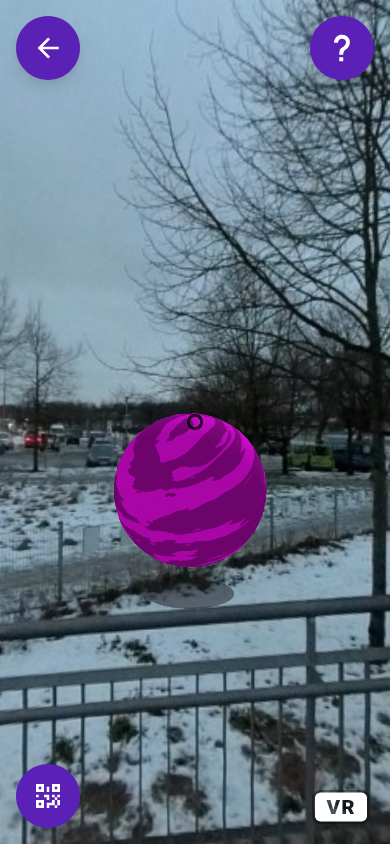
\includegraphics[width=.6\linewidth]{emi_ar-2.png}
    \end{minipage}
    \caption{\ac{AR}/\ac{VR} Szene während des virtuellen Besuchs}
    \label{fig:emi-ar}
\end{figure}

\begin{figure}[htpb]
    \begin{minipage}{.5\textwidth}
        \centering
        
\includegraphics[width=.6\linewidth]{emi_project-1.png}
    \end{minipage}%
    \begin{minipage}{.5\textwidth}
        \centering
        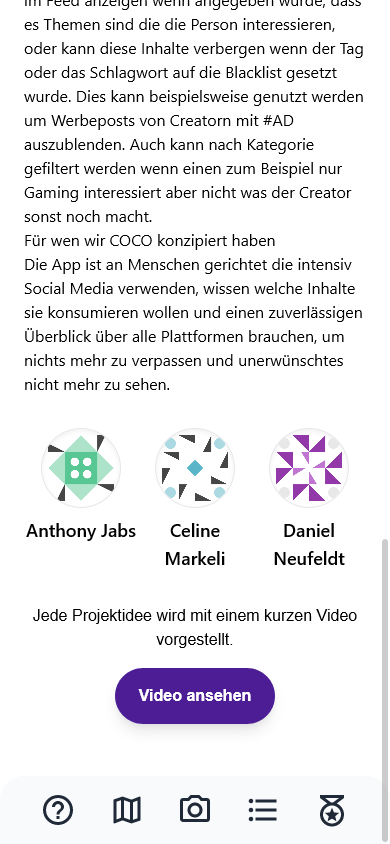
\includegraphics[width=.6\linewidth]{emi_project-2.png}
    \end{minipage}
    \caption{Einzelansicht eines Projekts}
    \label{fig:emi-project}
\end{figure}

Des Weiteren können verschiedene Abzeichen für bestimmte Aktionen erhalten
werden. Aktionen sind z. B. das Besuchen einer bestimmten Anzahl von Projekten
oder Benutzen von bestimmten Funktionen. Alle Abzeichen und ihr Fortschritt
können in einer Übersicht eingesehen werden (\autoref{fig:emi-achievments}).
Bestimmte Abzeichen werden in mehreren Stufen freigeschaltet oder bleiben bis
zum Erhalt verborgen. \\
Zudem werden die gesammelten „Awardteile“ angezeigt. Awardteile sind sammelbare
Objekte, welche auf der Karte mit einem Meteorit-Symbol
(\textgraphics{emi_meteorit.png}) gekennzeichnet sind. Beim Annähern an die
gezeigten Standorte wird eine Schaltfläche hervorgehoben, welche durch Antippen
das entsprechende Awardteil sammelt.

\begin{figure}[htpb]
    \centering
    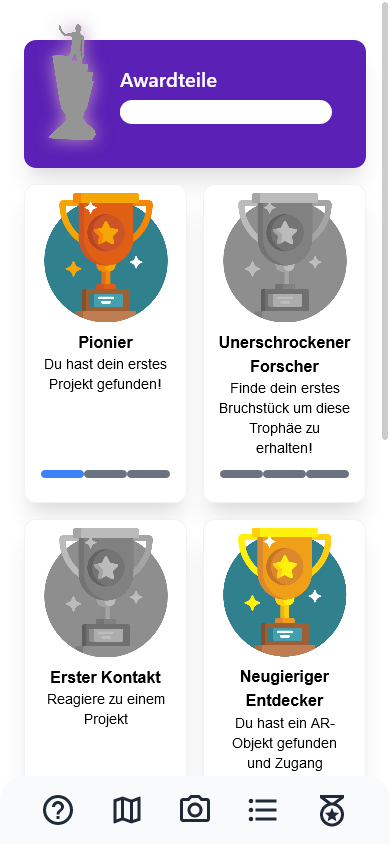
\includegraphics[width=.3\textwidth]{emi_achievements.png}
    \caption{Abzeichen- und Awardteilansicht}
    \label{fig:emi-achievments}
\end{figure}

Außerdem werden die genannten Funktionen in der App durch eine Slideshow
erklärt, welche jederzeit über die Navigationsleiste erreichbar ist (\autoref{fig:emi-help}).

\begin{figure}[htpb]
    \centering
    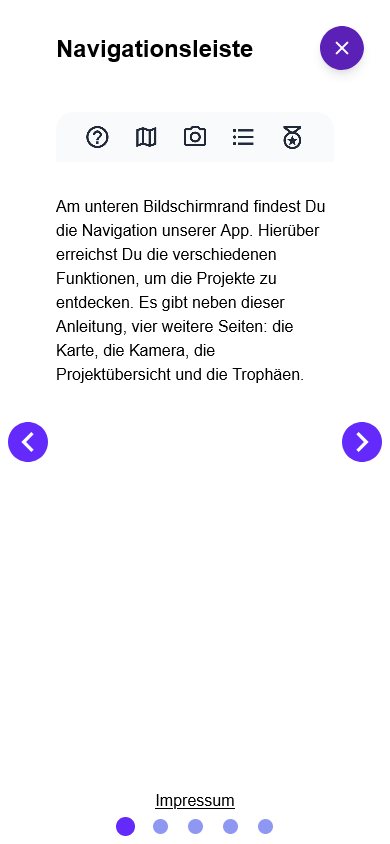
\includegraphics[width=.3\textwidth]{emi_help.png}
    \caption{Eine Seite der In-App-Anleitung}
    \label{fig:emi-help}
\end{figure}

Aus Veranstaltendensicht kann die EMI-Award-App rudimentär verwaltet werden.
Stationen, Abzeichen, Hilfseinträge, die Einführung und sammelbare Objekte
lassen sich über eine Web-Oberfläche eintragen und jederzeit verändern. Jedoch
werden Besuche und gesammelte Abzeichen vom System nicht erfasst und sind somit
nicht auswertbar. Auch die gesammelten Daten, darunter z. B. die Anzahl der
registrierten Teilnehmenden, sind nicht einsehbar. Zusammenfassend ergeben sich
daraus die in \autoref{table:emi-func} dargelegten Funktionalitäten.

\begin{table}[htpb]
    \def\arraystretch{1.25}
    \centering
    \caption{Funktionalitäten der EMI-Award-App}
    \label{table:emi-func}
    \begin{tabular}{ll}
        \uzlhline
        \uzlemph{ID} & \uzlemph{Funktionalität}                 \\
        \uzlhline%
        FT-Emi-1     & Interaktive Karte mit Stationen          \\
        FT-Emi-2     & Auflistung der Stationen                 \\
        FT-Emi-3     & Virtuelles Besuchen per QR-Code          \\
        FT-Emi-4     & Abzeichen                                \\
        FT-Emi-5     & Bedienungshilfe                          \\
        FT-Emi-6     & Einleitende Slideshow                    \\
        FT-Emi-7     & Rudimentäre Verwaltung der Informationen \\
        \uzlhline
    \end{tabular}
\end{table}

\newpage

\subsection{Analyse der Benutzeroberfläche} \label{ssec:analysis-old-ui}

In diesem Abschnitt werden mögliche Schwächen der Benutzeroberfläche untersucht,
um diese in der Konzeption adressieren zu können. Im Allgemeinen ist die
verwendete Schriftgröße der Benutzeroberfläche zu klein. Die empfohlene
Mindestschriftgröße beträgt 16 px für Smartphones im Abstand von 30 cm
\citedin{DIN1450}. Einige Teile der Benutzeroberfläche verwenden jedoch eine
Schriftgröße von nur 12 px.

Das Karten-Pop-up (\autoref{fig:emi-intro-map}) ist von diesem Problem
betroffen. Es verwendet eine Schriftgröße von 12 px und ist somit deutlich zu
klein. Des Weiteren nutzen Titel und Kurzbeschreibung identische Typografie. Der
Abstand ist ebenfalls identisch mit dem Zeilenabstand der Texte. Es liegt somit
kein visueller Unterschied zwischen Titel und Kurzbeschreibung vor. \\
Außerdem gibt es keinen Indikator dafür, ob die Station bereits besucht wurde.
Somit müssen Nutzer:innen sich den Besucht-Status in der Stationsliste anschauen
und merken, um auf der Karte darüber informiert zu sein. Dies steht im Gegensatz
zur 6. Usability Heuristik nach \textcite{Nielsen1994}, welche besagt, dass
Nutzer:innen nicht gezwungen sein sollten, sich Informationen zwischen Ansichten
zu merken. Stattdessen sollten die Informationen direkt ersichtlich sein.


\subsection{Analyse der technischen Umsetzung} \label{ssec:analysis-old-tech}

In der Analyse des Bachelorprojekts zur EMI-Award-App wurde festgestellt, dass
die Entwicklung einer nativen Android- und iOS-App einen höheren Aufwand in der
Entwicklung und Veröffentlichung darstellt \cite{Canzler2021}. Frameworks wie
Flutter \cite{Google2022} erleichtern die Entwicklung nativer Apps, indem der
gleiche Code für verschiedene Plattformen genutzt werden kann. Jedoch benötigt
die Entwicklung für iOS ein Gerät mit macOS \cite{Apple2022}. Die
Veröffentlichung der Apps erfordert zudem ein plattformspezifisches
(Apple/Google) Entwicklerkonto, über welches die Veröffentlichung der App
verwaltet wird. Im Gegensatz zu Web-Apps müssen die Veröffentlichung und
folgende Updates bei nativen Apps erst durch den Betreiber des jeweiligen
App-Stores überprüft und freigeschaltet werden.

Entsprechend wurde die EMI-Award-App als \ac{PWA} mit dem \textit{Vue.js}
\cite{You2022a} Framework realisiert und war unter \url{https://app.emi-award.de}
verfügbar. Zusätzlich wurden \textit{Mapbox} \cite{Mapbox2022} für die
interaktive Karte und \textit{A-Frame} \cite{Supermedium2021} für
\ac{AR}/\ac{VR}-Interaktion genutzt. Die Web-Oberfläche für Veranstaltende wurde basierend
auf \textit{Strapi} \cite{Strapi2022} entwickelt. Da der Fokus des zugehörigen
Bachelorprojekts auf der Entwicklung einer App für den EMI-Award lag, wurden die
Funktionalitäten speziell und nicht-anpassbar auf diesen zugeschnitten \cite{Canzler2021}. Somit
müssen sämtliche Teilsysteme überarbeitet werden, um diese für andere
Veranstaltungen zu verallgemeinern.


\section{Formalisierte Anforderungen} \label{sec:analysis-anf}

In diesem Abschnitt werden die systematisch formalisierten Anforderungen
dargelegt, welche die Ergebnisse der gesamten Analyse nach
\textcite{Balzert2009} zusammenfassen. Zu Beginn werden Visionen und darauf
aufbauende Ziele definiert. Zudem werden Rahmenbedingungen und Kontext des
Systems aufgezeigt. Anschließend werden die daraus resultierenden funktionalen
und qualitativen Anforderungen festgelegt.

\subsection{Vision und Ziele}

Die Grundlage der Anforderungen bilden die Visionen und Ziele des Systems. Das
Festlegen dieser erlaubt eine Überprüfung der Zielgerichtetheit der
Anforderungen \cite{Balzert2009}. Diese leiten sich aus den Zielen der Arbeit
(\autoref{sec:goals}), sowie der vorangegangenen Analyse der Organisation,
Benutzenden und Problemen ab. Den Anfang bilden die Visionen, welche
realitätsnah Vorstellungen der Zukunft darstellen.

\setanf{V}
\begin{center}
    \def\arraystretch{1.5}
    \begin{tabular}{m{0.08\textwidth}m{0.85\textwidth}}
        \uzlhline
        \anfrow & Veranstaltende sind besser in der Lage, ihre
        Veranstaltung zu planen, überblicken und auszuwerten.
        \\
        \anfrow & Veranstaltende sind besser in der Lage, mit
        Teilnehmenden zu kommunizieren.
        \\
        \anfrow & Teilnehmende werden motiviert und
        unterstützt, sich in der Veranstaltung zurechtzufinden.
        \\
        \anfrow & Teilnehmende können auf Wunsch der Veranstaltenden dazu
        motiviert werden, sich sozial auszutauschen
        \\
        \uzlhline
    \end{tabular}
\end{center}

Auf Basis der Visionen werden Ziele formuliert, welche die Visionen
operationalisieren. Diese folgen dabei den standardisierten Regeln zur
Formulierung von Zielen \cite{Pohl2008}.

\setanf{Z}
\begin{center}
    \def\arraystretch{1.5}
    \begin{longtable}{m{0.08\textwidth}m{0.85\textwidth}}
        \uzlhline
        \anfrow    & Veranstaltende sollen jederzeit in der Lage sein, Informationen
        zentral einzupflegen und diese zu verändern, um effektiv auf
        Veränderungen einzugehen.
        \\
        \anfrow    & Veranstaltende und Teilnehmende sollen ab Beginn der Veranstaltung in der
        Lage sein, besser miteinander zu kommunizieren.                                        \\
        \anfsubrow & Veranstaltende sollen ab Beginn der Veranstaltung in der
        Lage sein, Teilnehmenden Benachrichtigungen zu senden, um diesen zeitnah
        mit wichtigen Informationen versorgen zu können.                                       \\
        \anfsubrow & Veranstaltende sollen ab Beginn der Veranstaltung in der
        Lage sein, Teilnehmende jederzeit um Feedback zu fragen, um Probleme
        frühzeitig zu erkennen.
        \\
        \anfsubrow & Teilnehmende sollen ab Beginn der Veranstaltung in der
        Lage sein, Veranstaltende unkompliziert und jederzeit zu kontaktieren.
        \\
        \anfrow    & Teilnehmende sollen ab Beginn der Veranstaltung in der
        Lage sein, sich über die Aktivitäten der Veranstaltung zu informieren,
        um die Navigation der Veranstaltung zu erleichtern.                                    \\
        \anfrow    & Teilnehmende sollen ab Beginn der Veranstaltung in der
        Lage sein, bei Schwierigkeiten schnell an hilfreiche Informationen zu
        gelangen.                                                                              \\
        \anfrow    & Teilnehmende sollen ab Beginn der Veranstaltung in der Lage
        sein, für ihre aktive Teilnahme belohnt zu werden.
        \\
        \anfrow    & Teilnehmende sollen in der Lage
        sein, die veranstaltungsbezogenen Aktivitäten mit anderen Personen gemeinsam abzuschließen
        \\
        \anfrow    & Das System soll Informationen zugänglich präsentieren.
        \\
        \anfrow    & Veranstaltende sollen in der Lage sein, das Design des
        Systems auf ihre Veranstaltung anzupassen.
        \\
        \anfrow    & Veranstaltende sollen jederzeit in der Lage sein, vom
        System gesammelte Daten übersichtlich und strukturiert einzusehen.                     \\
        \uzlhline
    \end{longtable}
\end{center}
\vspace{-3cm}

\subsection{Rahmenbedingungen}

Die Rahmenbedingungen legen organisatorische und technische Restriktionen für
das System oder den Entwicklungsprozess fest \cite{Balzert2009}. Die Bedingungen
wurden aus der Benutzer und Kontextanalyse, sowie der Analyse des bestehenden
Systems abgeleitet.

\setanf{R}
\begin{center}
    \def\arraystretch{1.5}
    \begin{longtable}{m{0.08\textwidth}m{0.85\textwidth}}
        \uzlhline
        \anfrow & Das System ist eine Web-Anwendung. (vgl. \ssecref{ssec:analysis-old-tech})
        \\
        \anfrow & Die Zielgruppen sind Personen, welche Veranstaltungen
        organisieren und Teilnehmende dieser Veranstaltungen. Die
        Nutzungsgruppen wurden in \autoref{sec:analysis-user} definiert.
        \\
        \anfrow & Das System wird von Veranstaltenden in einem
        Arbeitsplatzsystemkontext genutzt und von Teilnehmenden vorwiegend in
        einem mobilen Kontext genutzt.                                                     \\
        \anfrow & Das System wird über die Länge der Veranstaltung im
        Dauerbetrieb laufen.                                                               \\
        \anfrow & Das System soll auf Wunsch auch nach der
        Veranstaltung noch für beliebige Zeit erreichbar sein.                             \\
        \anfrow & Das System muss unbeaufsichtigt zuverlässig lauffähig
        sein.                                                                              \\
        \anfrow & Auf den Zielmaschinen verwendete Software:
        \newline
        Client:
        Moderne marktführende Webbrowser (Chrome, Firefox, Edge, Safari)
        \\
        \uzlhline
    \end{longtable}
\end{center}
\vspace{-3cm}

\subsection{Kontext und Überblick}

Jedes System ist in einer technischen Umgebung eingebettet \cite{Balzert2009}.
Im Folgenden wird Bezug auf das aktuelle System genommen.

\setanf{K}
\begin{center}
    \def\arraystretch{1.5}
    \begin{tabular}{m{0.08\textwidth}m{0.85\textwidth}}
        \uzlhline
        \anfrow & Das aktuelle System ist eine Web-Anwendung, welche die
        Grundlage des neuen Systems darstellt.
        \\
        \uzlhline
    \end{tabular}
\end{center}
\vspace{-1cm}

\subsection{Funktionale Anforderungen} \label{ssec:analysis-anf-func}

Die funktionalen Anforderungen halten die Kernfunktionalitäten des Systems fest
\cite{Balzert2009}. Diese ergeben sich aus allen Teilanalysen und den
festgelegten Zielen. Um eine eindeutige Semantik bei natürlichsprachlichen
Anforderungen zu gewährleisten, wird eine Anforderungsschablone (\autoref{fig:anf-schablone}) verwendet,
welche die Anforderungen vereinheitlicht \cite{Balzert2009}.

\begin{figure}[htpb]
    \renewcommand\baselinestretch{1}
    \centering
    \tikzset{
        textbox/.style={
                minimum height=1.75cm,
                text centered,
                align=center
            },
        small/.style={
                text width=1.9cm,
            },
        medium/.style={
                text width=2.5cm,
            },
        big/.style={
                text width=2.92cm,
            },
        arrow/.style={
                -
            },
        every node/.style={scale=0.8},
    }
    \tikz [thesis box shapes, baseline, anchor=base, scale=0.8]{
        \coordinate (origin);

        \node [block] (1a) [textbox, medium, right=of origin] {\textbf{Element}\linebreak„Die Komponente <Name>“};
        \node [block] (1b) [textbox, medium, above=0.35cm of 1a] {\textbf{Element}\linebreak„Das System“};

        \coordinate [right=0.175cm of {$(1a.east)!0.5!(1b.east)$}] (1X);

        \node [block] (2a) [textbox, small, right=0.175cm of 1X] {\textbf{Mittlere Priorität}\linebreak„soll“};
        \node [block] (2b) [textbox, small, above=0.35cm of 2a] {\textbf{Hohe Priorität}\linebreak„muss“};
        \node [block] (2c) [textbox, small, below=0.35cm of 2a] {\textbf{Niedrige Priorität}\linebreak„sollte in Zukunft“};

        \coordinate [right=0.175cm of 2a] (2X);

        \node [block] (3a) [textbox, big, right=0.175cm of 2X] {\textbf{Benutzerinteraktion}\linebreak„<Wem> die Möglichkeit bieten“};
        \node [block] (3b) [textbox, big, above=0.35cm of 3a] {\textbf{Selbstständige Systemaktivität}\linebreak„“};
        \node [block] (3c) [textbox, big, below=0.35cm of 3a] {\textbf{Schnittstellenanforderungen}\linebreak„fähig sein“};

        \node [block] (4) [textbox, medium, right=0.35cm of 3a] {\textbf{Bezug}\linebreak„<Objekt \& Ergänzung des Objektes>“};

        \node [block] (5) [textbox, medium, right=0.35cm of 4, yshift=-2cm] {\textbf{Bei Qualitätsanforderungen}\linebreak„<Qualität>“};

        \node [block] (6) [textbox, medium, right=0.35cm of 5, yshift=2cm] {\textbf{Funktionalität}\linebreak„<Prozesswort>“};

        \draw[arrow] (1a.east) to (1X);
        \draw[arrow] (1b.east) to (1X);
        \draw[arrow] (1X) to (2a.west);
        \draw[arrow] (1X) to (2b.west);
        \draw[arrow] (1X) to (2c.west);

        \draw[arrow] (2a.east) to (2X);
        \draw[arrow] (2b.east) to (2X);
        \draw[arrow] (2c.east) to (2X);
        \draw[arrow] (2X) to (3a.west);
        \draw[arrow] (2X) to (3b.west);
        \draw[arrow] (2X) to (3c.west);

        \draw[arrow] (3a.east) to (4.west);
        \draw[arrow] (3b.east) to (4.west);
        \draw[arrow] (3c.east) to (4.west);

        \draw[arrow] (4.east) to (5.west);
        \draw[arrow] (4.east) to (6.west);

        \draw[arrow] (5.east) to (6.west);
    }
    \caption{Anforderungsschablone \cite{Balzert2009}}
    \label{fig:anf-schablone}
\end{figure}

% TODO: Anfang und Ende Funktion als Anforderung

\setanf{F}
\begin{center}
    \def\arraystretch{1.5}
    \begin{longtable}{m{0.08\textwidth}m{0.85\textwidth}}
        \uzlhline
        \anfrow    & Das System \textit{muss} Veranstaltenden die
        Möglichkeit bieten, veranstaltungsrelevante Informationen einzutragen
        und jederzeit zu verändern (\anfref{Z10}).                                   \\
        \anfsubrow & Das System \textit{muss} Veranstaltenden die
        Möglichkeit bieten, Stationen einzutragen und jederzeit zu verändern.        \\
        \anfsubrow & Das System \textit{muss} Veranstaltenden die
        Möglichkeit bieten, Abzeichen einzutragen und jederzeit zu verändern.        \\
        \anfsubrow & Das System \textit{muss} Veranstaltenden die
        Möglichkeit bieten, Hilfe (FAQ) jederzeit einzutragen oder zu verändern.
        \\
        \anfsubrow & Das System \textit{muss} Veranstaltenden die
        Möglichkeit bieten, einführende Folien (Intro) jederzeit einzutragen
        oder zu verändern.
        \\
        \anfrow    & Das System \textit{muss} Veranstaltenden die Möglichkeit
        bieten, Statistiken zu den veranstaltungsbezogenen Aktivitäten
        einzusehen (\anfref{Z80}).                                                   \\
        \anfrow    & Das System \textit{muss} Teilnehmenden ab Beginn der
        Veranstaltung die Möglichkeit bieten, jederzeit Informationen
        einzusehen (\anfref{Z30}).
        \\
        \anfrow    & Das System \textit{muss} Teilnehmenden ab Beginn der
        Veranstaltung die Möglichkeit bieten, eine Einführung in den Kontext der
        Veranstaltung zu erhalten (\anfref{Z30}).
        \\
        \anfrow    & Das System \textit{muss} Teilnehmenden ab Beginn der
        Veranstaltung die Möglichkeit bieten, jederzeit hilfreiche Einträge bei Fragen einzusehen (\anfref{Z40}).
        \\
        \anfrow    & Das System \textit{muss} Teilnehmenden ab Beginn der
        Veranstaltung die Möglichkeit bieten, Abzeichen für bestimmte Handlungen
        zu verleihen (\anfref{Z50}).                                                 \\
        \anfrow    & Das System \textit{muss} Veranstaltenden die
        Möglichkeit bieten, Teilnehmenden jederzeit Benachrichtigungen zu
        senden (vgl. \autoref{sec:analysis-context}, \anfref{Z21}).
        \\
        \anfrow    & Das System \textit{soll} Veranstaltenden die Möglichkeit
        bieten, Teilnehmende jederzeit um Feedback bitten (vgl.
        \autoref{sec:analysis-context}, \anfref{Z22}).                        \\
        \anfrow    & Das System \textit{soll} Veranstaltenden die
        Möglichkeit bieten, die Rahmendaten der Veranstaltung jederzeit
        einzutragen oder zu ändern (\anfref{Z10}).
        \\
        \anfrow    & Das System \textit{soll} Teilnehmenden die Möglichkeit
        bieten, als Gruppe Stationen zu besuchen und Abzeichen abzuschließen.        \\
        \anfrow    & Das System \textit{sollte in Zukunft} fähig sein,
        Informationen in verschiedenen Sprachen darzustellen (\anfref{Z70}).         \\
        \anfrow    & Das System \textit{sollte in Zukunft} Teilnehmenden die
        Möglichkeit bieten, Veranstaltende jederzeit zu kontaktieren (\anfref{Z23}). \\
        \anfrow    & Das System \textit{sollte in Zukunft} umfassende
        Möglichkeiten zur Anpassung der Signalfarbe an die eigene Veranstaltung
        zulassen (\anfref{Z70}).
        \\
        \uzlhline
    \end{longtable}
\end{center}
\vspace{-3cm}

\subsection{Qualitätsanforderungen}

Abschließend werden Qualitätsanforderungen (auch nicht-funktionale
Anforderungen) festhalten. Diese legen qualitative oder quantitative
Eigenschaften des Systems fest \cite{Balzert2009}. Auch hier wird sich stark an
der Anforderungsschablone (\autoref{fig:anf-schablone}) orientiert.

\setanf{Q}
\begin{center}
    \def\arraystretch{1.5}
    \begin{longtable}{m{0.08\textwidth}m{0.85\textwidth}}
        \uzlhline
        \anfrow & Das System \textit{muss} den Grundsätzen der DIN EN ISO
        9241-110:2019-09 (Ergonomie der Mensch-System-Interaktion - Teil 110:
        Interaktionsprinzipien) folgen (\cite{DINISO9241}).                                                              \\
        \anfrow & Das System \textit{muss} die definierten Nutzungsklassen
        aus \autoref{sec:analysis-user} (Veranstaltende und Teilnehmende)
        unterscheiden und die dazugehörigen Zugriffsrechte sicherstellen.
        \\
        \anfrow & Das System \textit{muss} zuverlässig und ohne Störung im Dauerbetrieb laufen.
        \\
        \anfrow & Das System \textit{muss} die zehn Usability Heuristiken
        \cite{Nielsen1994} beachten. (\anfref{Z60})
        \\
        \anfrow & Das System \textit{soll} die Richtlinien des Deutschen
        Blinden- und Sehbehindertenverbandes berücksichtigen \cite{DBSV2022}.
        \\
        \anfrow & Das System soll weitestgehend auch offline
        genutzt werden können. (z. T. durch \anfref{Q30} und Herausforderungen
        der räumlichen Dimension, wie z. B. Mobilempfang)
        \\
        \anfrow & Das System \textit{soll} beim Zugriff über das Internet eine gesicherte Übertragung (HTTPS) ermöglichen.
        \\
        \anfrow & Das System \textit{soll} alle Benutzerinteraktionen in unter fünf Sekunden ausführen.
        \\
        \uzlhline
    \end{longtable}
\end{center}

% Während der Veranstaltung Fokus Überwachung und Sicherstellung der Aktivitäten
% -> Die Stationsdashboards mit Nachrichten, Informationen und Übersicht zur
% Überwachung

% Mobiler Einsatz -> Betriebssysteme für Handys
%   - iOS vs Android https://gs.statcounter.com/os-market-share/mobile/europe/
%   - PWA / Web-App

% Stabilität und Zuverlässigkeit *sehr* wichtig
%   - Ausfall kann gesamtes Event lahmlegen
%   - Bei hoher Teilnehmeranzahl hohe Last

% Warum inclusive Design
%   - Menschen aller gesellschaftlichen Schichten nehmen an Veranstaltungen teil
%   - Jedem sollte die Chance geboten werden teilzunehmen

% Gruppengefühl, Soziale Interaktion -> Gruppenfunktion, Reaktionen

% Bessere Kommunikation -> Stationsdashboard